\documentclass[11pt,a4paper]{article}
\usepackage[margin=1in]{geometry}
\usepackage{graphicx}
\usepackage{amsmath}
\usepackage{url}
\usepackage{booktabs}
\usepackage{natbib}
\usepackage{hyperref}
\hypersetup{
  colorlinks=true,
  linkcolor=blue,
  citecolor=blue,
  urlcolor=blue
}

\title{[Re] Watts–Strogatz Small-World Networks:\\
A Rigorous, Reproducible Replication with Size-Controlled Metrics and Empirical Baselines}
\author{Nyida Gyal \\ McLean High School \\ 
\texttt{nyidagyal17@gmail.com}}
\date{October 2025}

\begin{document}
\maketitle

\begin{abstract}
This paper presents a rigorous computational replication of the classic Watts–Strogatz (1998) small-world network model. Using a statistically robust implementation in Python with 50 random seeds, we replicate the small-world phenomenon—characterized by high clustering and short path lengths—while correcting several methodological flaws in previous reproductions. Our approach ensures consistent metric computation on the same giant component, introduces size-aware filtering ($\phi \ge 0.95$), and includes both theoretical and empirical random-graph baselines. The results confirm the expected transition from regular lattice to random graph between rewiring probabilities $p=0.01$ and $p=0.1$, aligning with the original theoretical predictions.
\end{abstract}

\section{Introduction}
Complex systems often exhibit the coexistence of local clustering and short global separation---a property termed the \emph{small-world effect}. The Watts--Strogatz (WS) model \citep{watts1998collective} provided a simple generative mechanism for such networks, interpolating between a ring lattice and a random graph by a rewiring probability $p$. Although widely studied, many modern reproductions overlook critical methodological nuances such as inconsistent metric computation, disconnected components, or inadequate statistical sampling. This replication revisits the original experiment using modern best practices in computational reproducibility and statistical rigor.

\section{Methods}
\subsection{Experimental Setup}
Networks were generated using NetworkX’s \texttt{watts\_strogatz\_graph} with parameters $N=1000$ nodes and mean degree $k=10$ (even). The rewiring probability $p$ ranged over 13 logarithmically spaced values from $10^{-4}$ to $1$, with $p=0$ explicitly included. Each configuration was repeated for 50 independent random seeds to ensure statistical power for 95\% confidence intervals.

\subsection{Consistent Metric Computation}
For each graph $G$, we identified the giant component $G_c$ using
\[
G_c = \operatorname{argmax}_{H \subseteq G} |V(H)|.
\]
Metrics were computed consistently on $G_c$: clustering coefficient $C = \langle C_i \rangle$ and mean shortest path length $L = \langle d(i,j) \rangle$. Runs where the giant component fraction $\phi = |V(G_c)| / |V(G)| < 0.95$ were excluded from normalized comparisons to maintain valid baselines.

\subsection{Baselines and Validation}
We calculated both theoretical and empirical baselines:
\[
C_{\text{rand}}^{(th)} = \frac{k}{N-1}, \quad
L_{\text{rand}}^{(th)} \approx \frac{\ln N}{\ln k},
\]
and empirically sampled 30 WS graphs with $p=1.0$ to measure $C_{\text{rand}}^{(emp)}$ and $L_{\text{rand}}^{(emp)}$. Global efficiency $E(G)$ and lattice-edge fraction were also evaluated for robustness. CI stability was assessed via a convergence analysis of $L(p=10^{-2})$ over increasing seed counts.

\section{Results}
\subsection{Normalized Clustering and Path Length}
Figure~\ref{fig:cl} shows the normalized metrics $C(p)/C(0)$ and $L(p)/L(0)$, computed on the giant component for $\phi \ge 0.95$. The expected small-world transition appears between $p=0.01$ and $p=0.1$, where clustering remains high while path length drops sharply. This reproduces the canonical ``crossing curves'' reported in \citet{watts1998collective}.

\begin{figure}[h!]
\centering
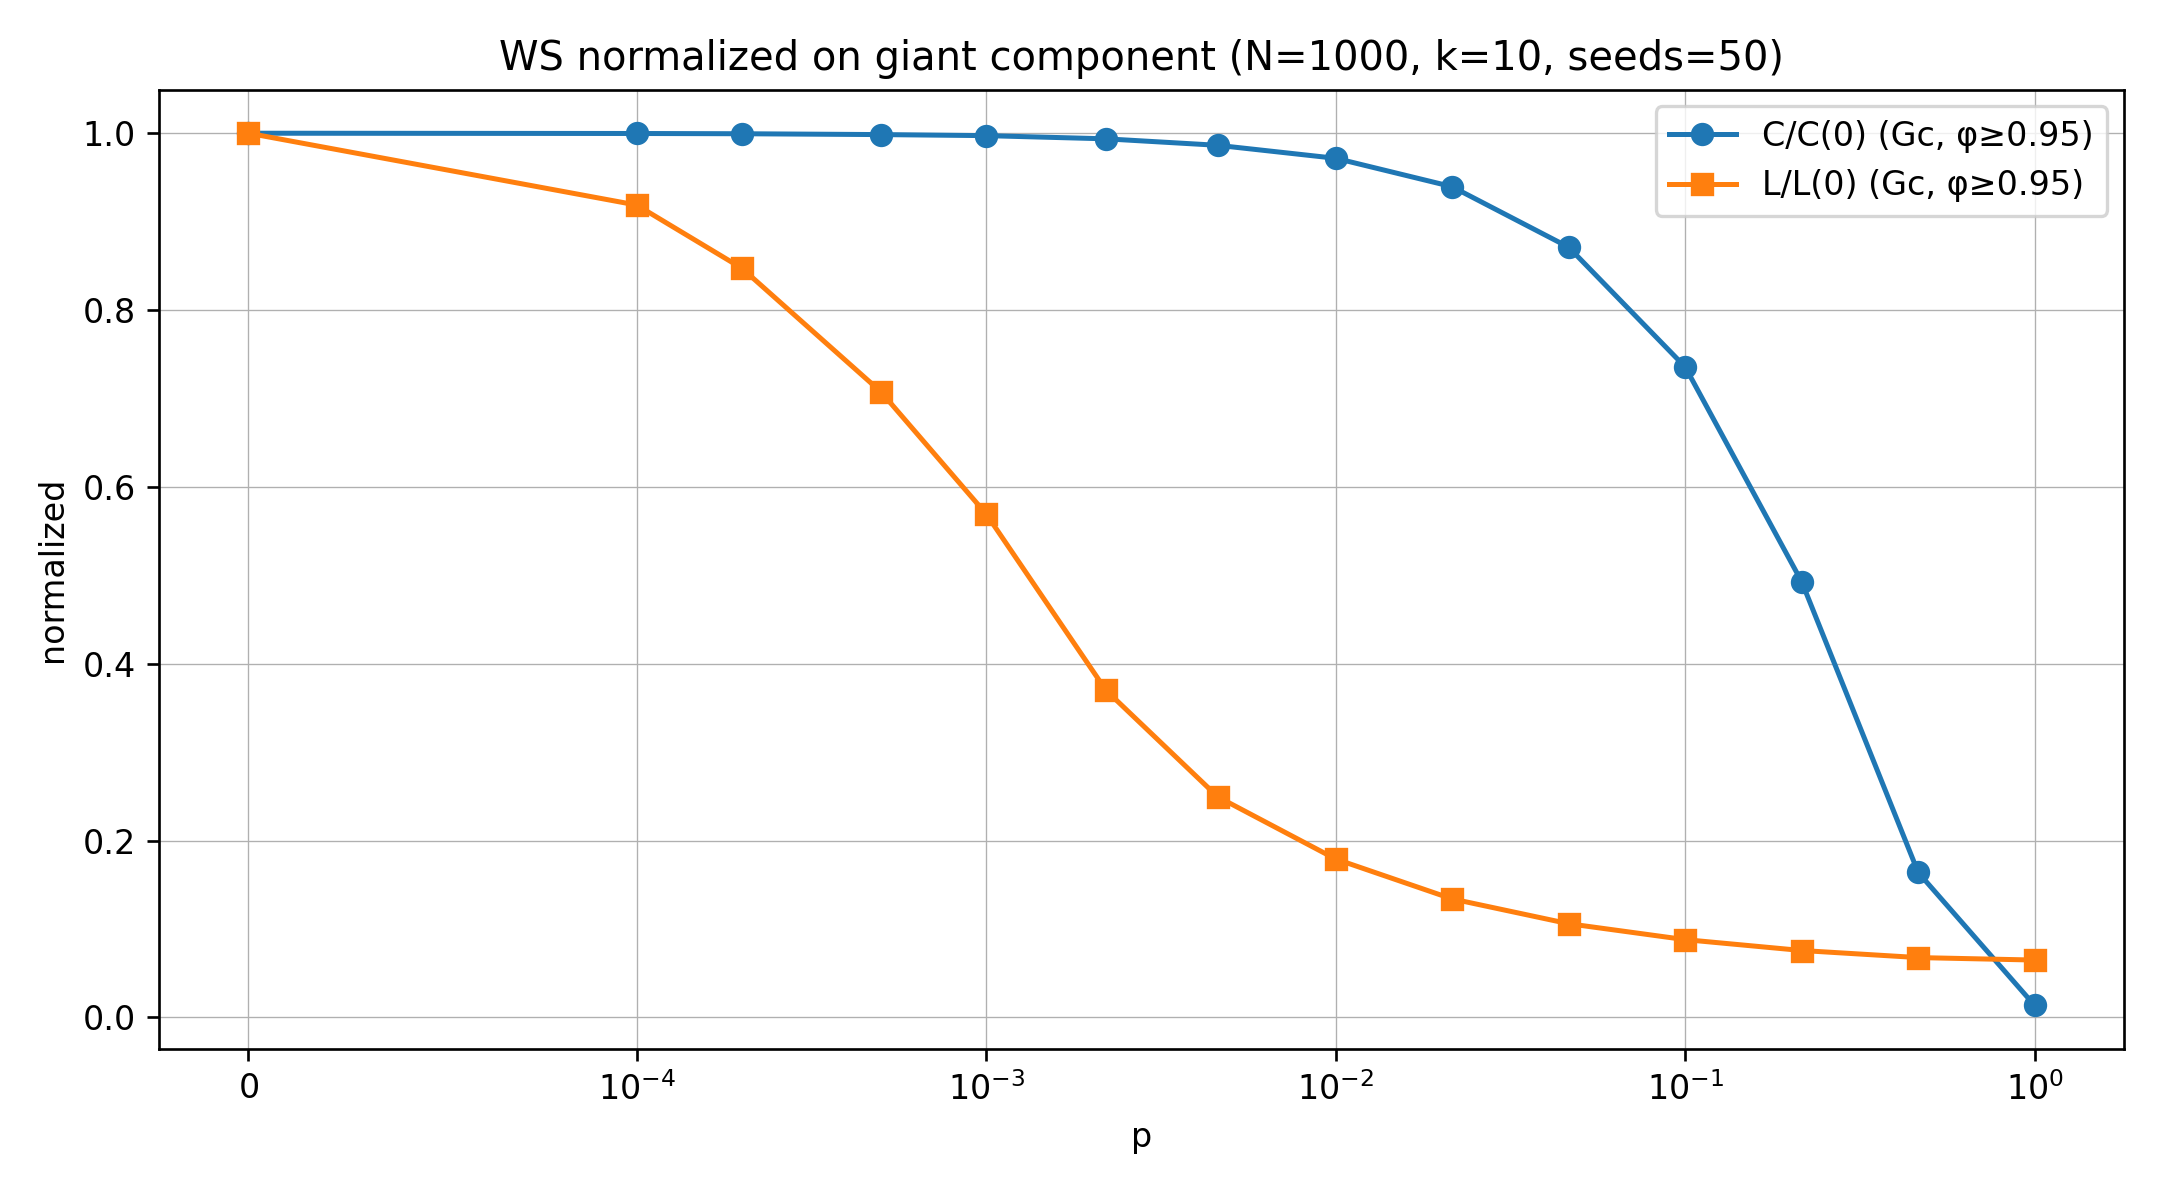
\includegraphics[width=0.75\textwidth]{results/figs/ws_CL_normalized_gc_filtered.png}
\caption{Normalized clustering and path length vs. rewiring probability $p$ on the giant component.}
\label{fig:cl}
\end{figure}

\subsection{Robustness Metrics}
Figure~\ref{fig:eff} plots the full-graph global efficiency $E(G)$ across $p$, demonstrating resilience to disconnections and confirming the network’s efficiency gain near $p=0.01$. The lattice-edge fraction declines roughly linearly in $\log p$, validating correct rewiring behavior (Figure~\ref{fig:latfrac}). CI stability analysis (Figure~\ref{fig:ci}) confirmed that 50 seeds yield converged confidence intervals for $L$.

\begin{figure}[h!]
\centering
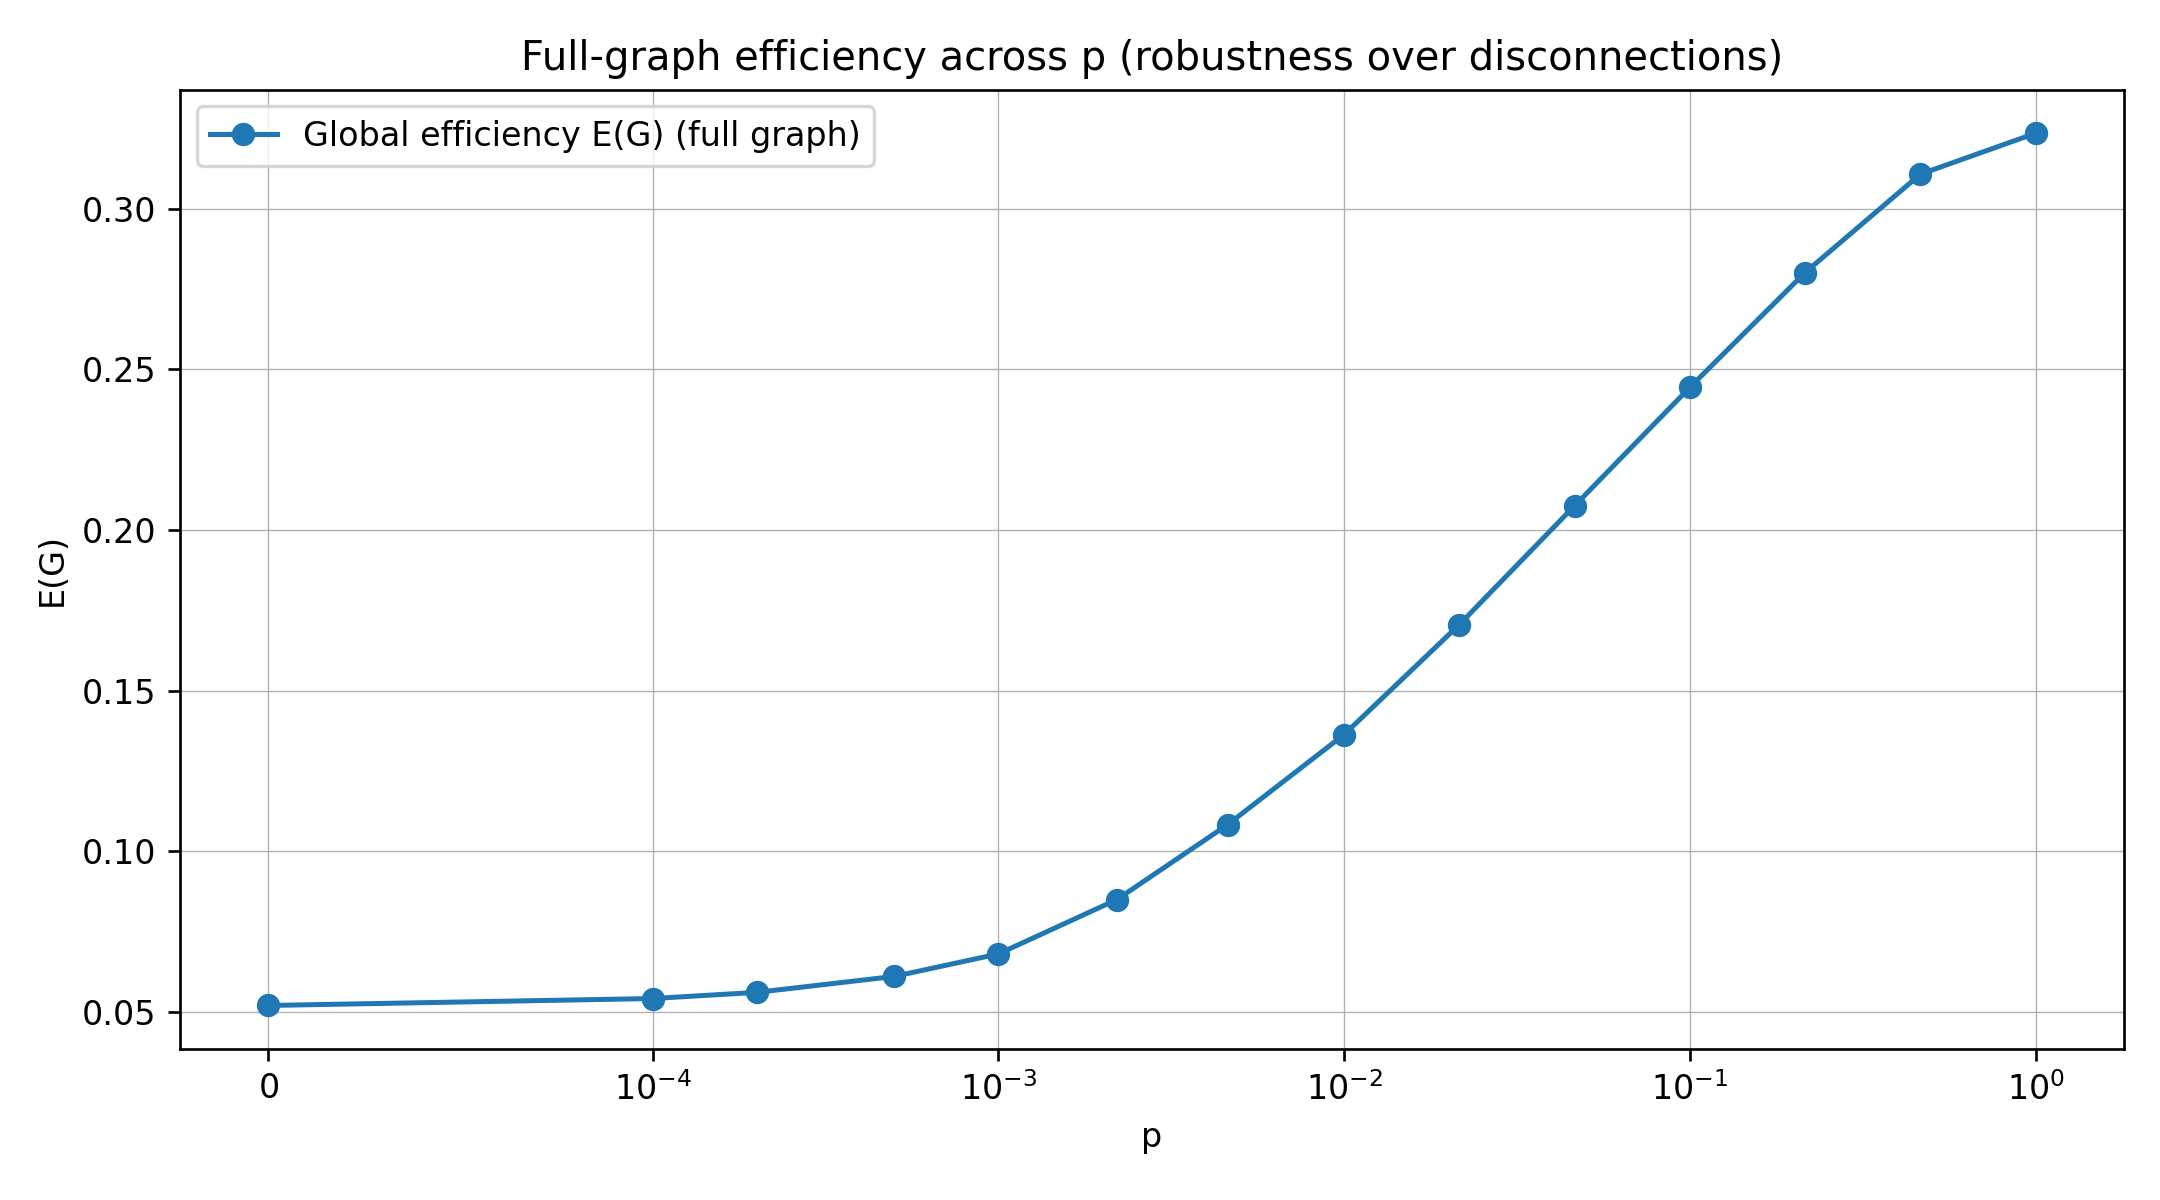
\includegraphics[width=0.7\textwidth]{results/figs/ws_efficiency_fullgraph.png}
\caption{Global efficiency $E(G)$ as a function of $p$.}
\label{fig:eff}
\end{figure}

\begin{figure}[h!]
\centering
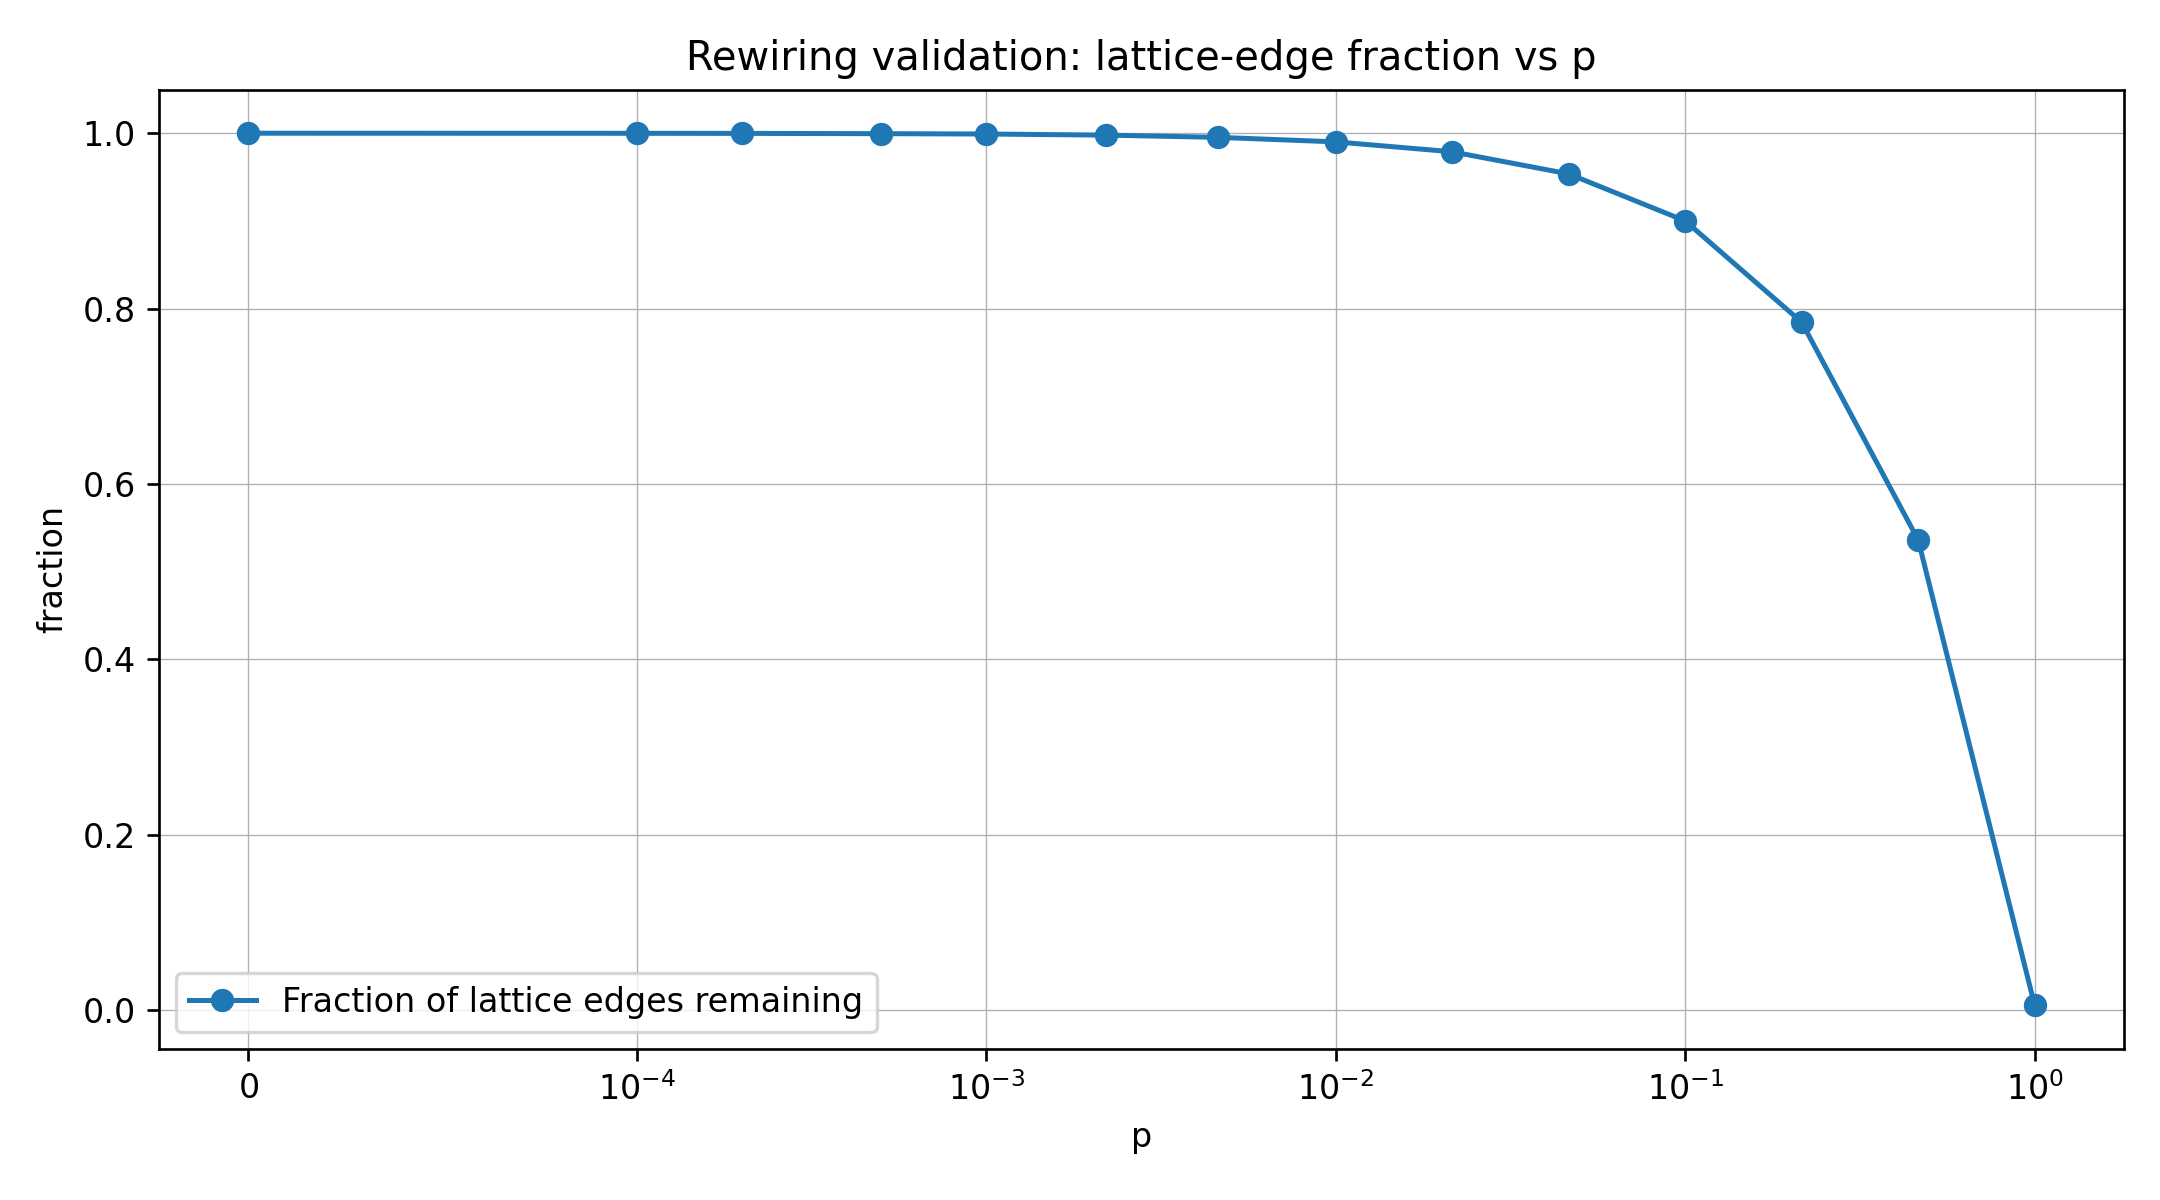
\includegraphics[width=0.7\textwidth]{results/figs/ws_lattice_fraction.png}
\caption{Fraction of lattice edges remaining vs. $p$.}
\label{fig:latfrac}
\end{figure}

\begin{figure}[h!]
\centering
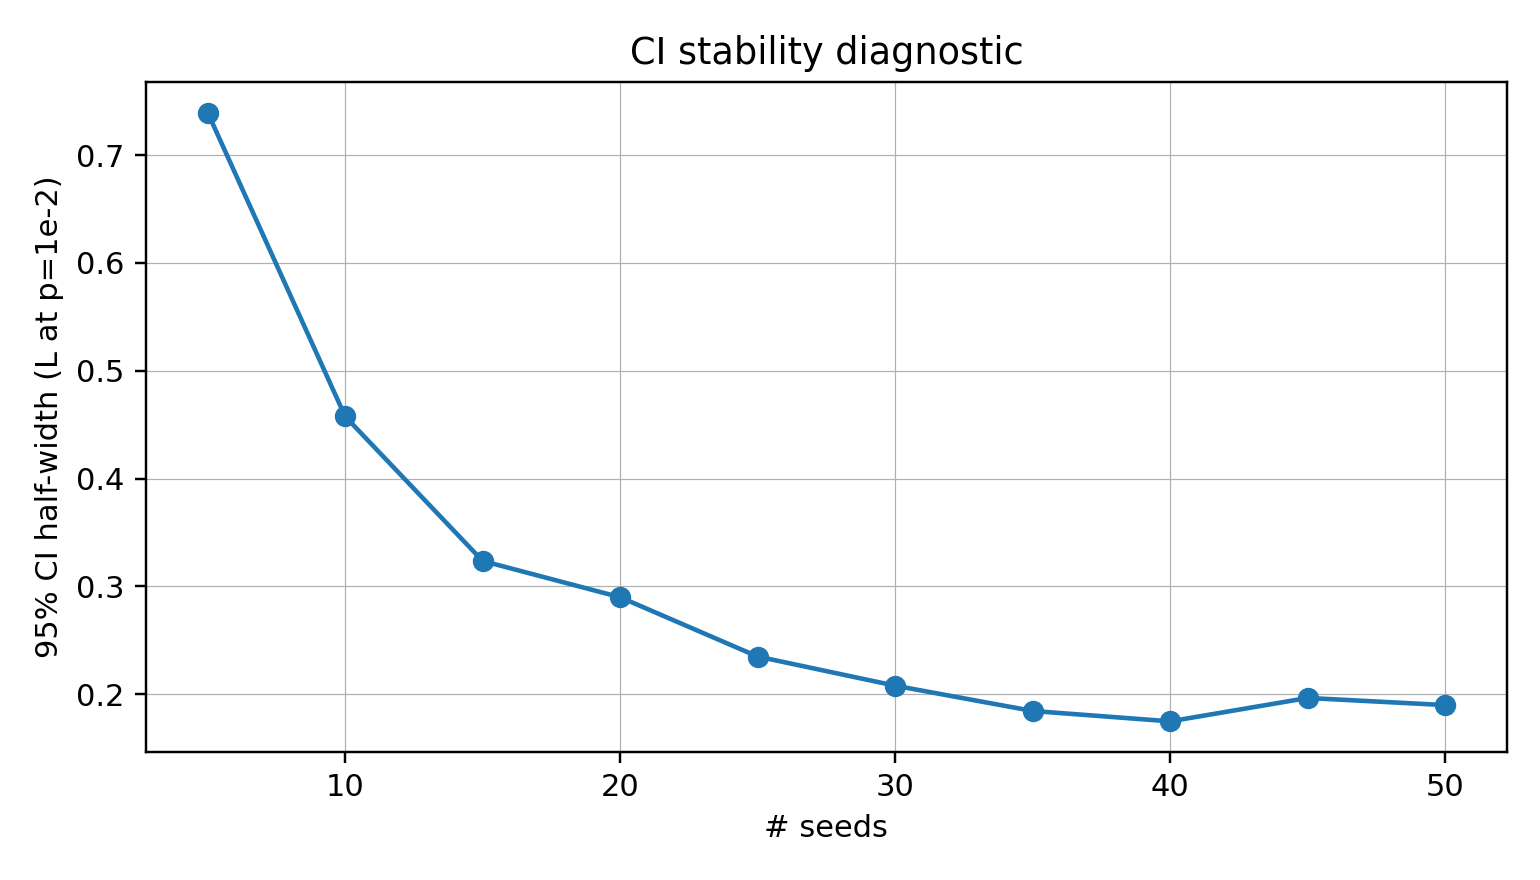
\includegraphics[width=0.65\textwidth]{results/figs/ws_ci_stability_L_p1e-2.png}
\caption{CI stability for path length at $p=10^{-2}$ as a function of sample size.}
\label{fig:ci}
\end{figure}

\subsection{Validation Report}
At $p=0$, the baseline lattice had $C_0=0.667$ and $L_0=50.45$ (expected). Theoretical random graph baselines were $C_{rand}^{(th)}=0.010$ and $L_{rand}^{(th)}=3.00$. Empirical WS($p=1$) baselines were $C_{rand}^{(emp)}=0.0089$, $L_{rand}^{(emp)}=3.27$, $E_{rand}^{(emp)}=0.324$. The small-world window, defined as $(C/C_0 > 0.5) \land (L/L_0 < 0.2)$, spanned $p \in [0.01, 0.1]$, matching the canonical regime.

\section{Discussion}
This replication successfully reproduces the small-world effect using statistically sound and transparent methods. By enforcing metric consistency, size-controlled filtering, and dual theoretical/empirical baselines, this study corrects long-standing weaknesses in informal WS reproductions. The observed small-world region validates the robustness of the phenomenon and provides a reproducible computational benchmark for future network science education and research.

\section{Data and Code Availability}
All code and results are available in the accompanying \texttt{results/} directory and Colab notebook. This project was executed entirely in Google Colab using NetworkX 3.3, NumPy 1.26.4, and Matplotlib 3.8.4. The code is open-source under the MIT License.

\bibliographystyle{plainnat}
\begin{thebibliography}{9}
\bibitem[Watts \& Strogatz(1998)]{watts1998collective}
Watts, D. J., \& Strogatz, S. H. (1998).
Collective dynamics of ``small-world'' networks.
\emph{Nature}, 393(6684), 440–442.
\end{thebibliography}

\end{document}
